\begin{multicols}{2}
\subsubsection*{Performance Evaluation} \label{sec:R:fitts}
This section will present the results acquired from the Fitts' Law target reaching test. The test had five metrics which each express a parameter of subjects performance. Subjects were divided into two groups, one test group which received continuous classifications scores during user training, and a control group which received binary classification scores during user training. The results have been plotted for each metric over all four sessions, with mean and standard deviations.
\end{multicols}




%throughput
\begin{figure}[H] 
	\subfigure[Throughput metric for the Fitts' Law test between the test and control group.]
	{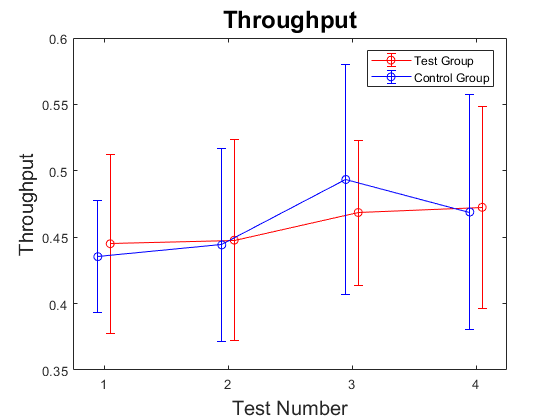
\includegraphics[width=.42\textwidth]{figures/xWesulds/Throughput}} 
\end{figure}


\begin{figure}[H] 
	\centering
	\subfigure[Path efficiency metric for the Fitts' Law test between the test and control group.]
	{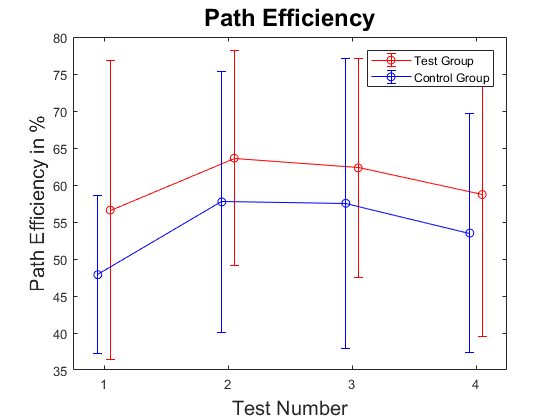
\includegraphics[width=.42\textwidth]{figures/xWesulds/PathEfficiency}} 
	\subfigure[Overshoot metric for the Fitts' Law test between the test and control group. There is no significant difference between the groups ($p > 0.05$).]
	{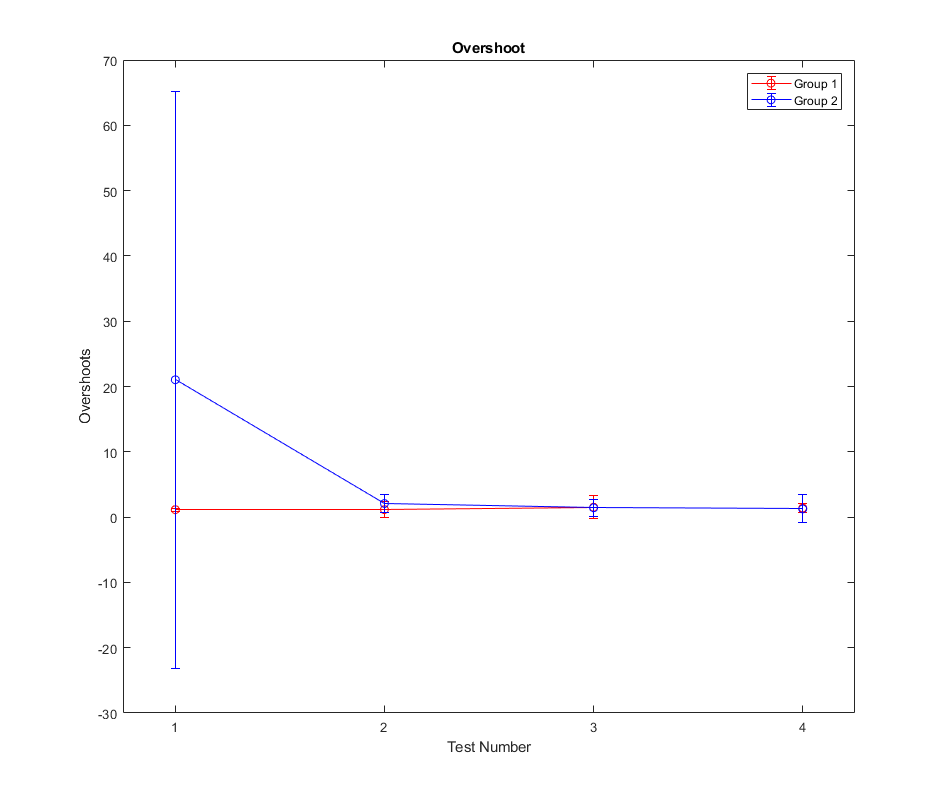
\includegraphics[width=.42\textwidth]{figures/xWesulds/Overshoot}}  

\end{figure}


\begin{figure}[H] 
	\centering
	\subfigure[Stopping distance metric for the Fitts' Law test between the test and control group. There is no significant difference between the groups ($p > 0.05$).]
	{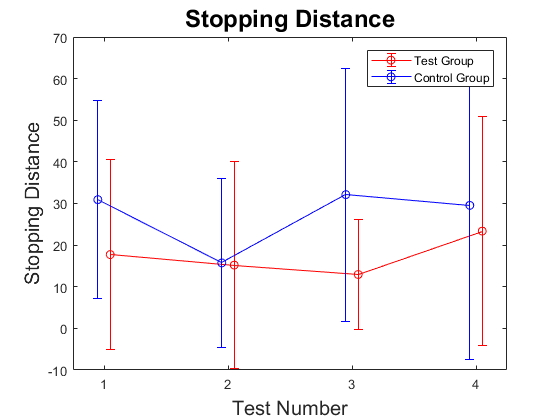
\includegraphics[width=.42\textwidth]{figures/xWesulds/StoppingDistance}} 
	\subfigure[Completion rate metric for the Fitts' Law test between the test and control group. There is no significant difference between the groups ($p > 0.05$).]
	{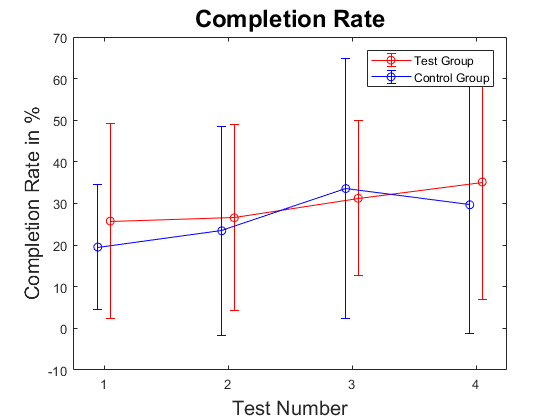
\includegraphics[width=.42\textwidth]{figures/xWesulds/CompletionRate}}  

\end{figure}



%
%%Path Efficiency
%\begin{figure}[H] 
%	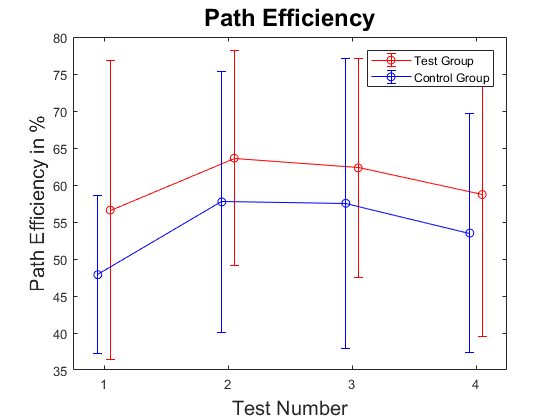
\includegraphics[width=0.3\textwidth]{figures/xWesulds/PathEfficiency}
%	\caption{Path efficiency metric for the Fitts' Law test between the test and control group.}
%	\label{fig:PEresult}
%\end{figure} 
%
%overshoot
%\begin{figure}[H] 
%	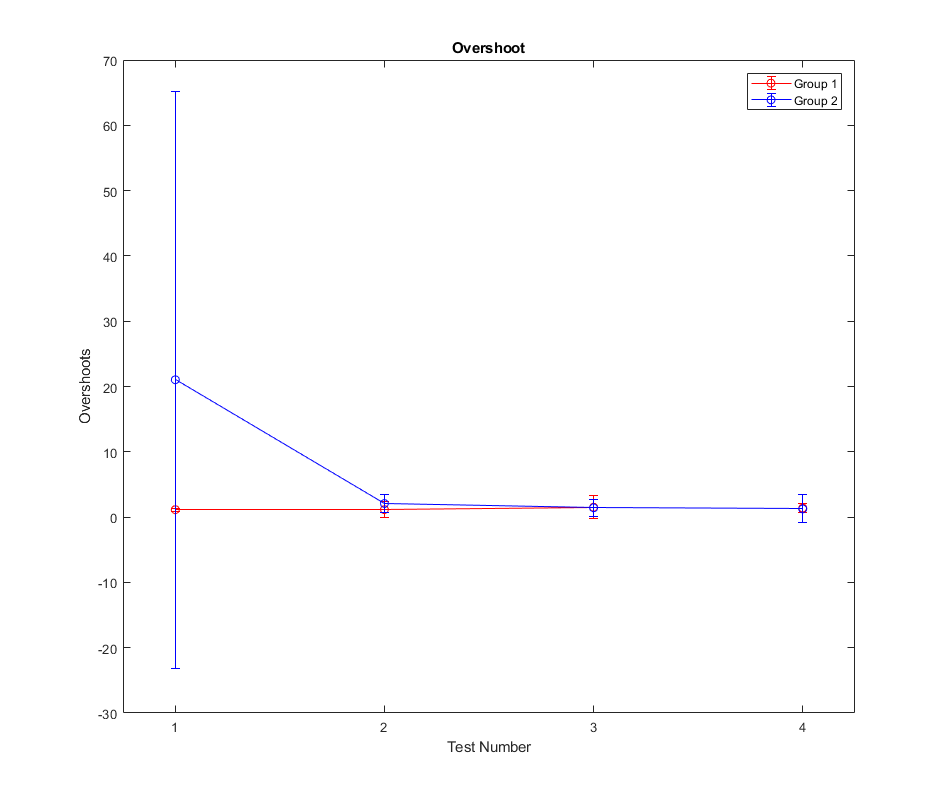
\includegraphics[width=0.3\textwidth]{figures/xWesulds/Overshoot}
%	\caption{Overshoot metric for the Fitts' Law test between the test and control group. There is no significant difference between the groups ($p > 0.05$).}
%	\label{fig:OSresult}
%\end{figure} 

%stopping distance
%\begin{figure}[H] 
%	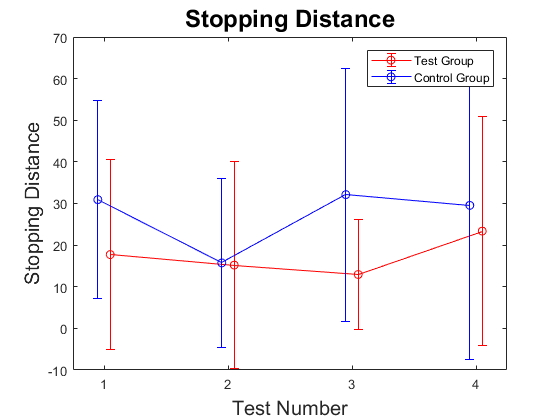
\includegraphics[width=0.3\textwidth]{figures/xWesulds/StoppingDistance}
%	\caption{Stopping distance metric for the Fitts' Law test between the test and control group. There is no significant difference between the groups ($p > 0.05$).}
%	\label{fig:SDresult}
%\end{figure} 
%
%%completion rate
%\begin{figure}[H] 
%	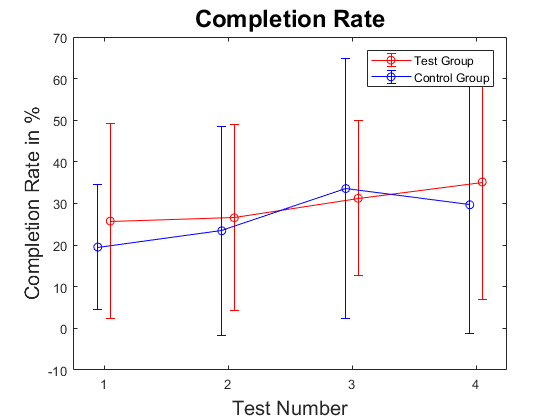
\includegraphics[width=0.3\textwidth]{figures/xWesulds/CompletionRate}
%	\caption{Completion rate metric for the Fitts' Law test between the test and control group. There is no significant difference between the groups ($p > 0.05$).}
%	\label{fig:CRresult}
%\end{figure} 
\begin{multicols}{2}
	
The Fitts' Law results did not show any significant change over the three sessions for any of the five test metrics, with all comparisons within both the test and control group resulting in p-values above $0.05$, with a Tukey-Kramer correction yielding p-values above $0.05$ for all comparisons within both groups. At the same time there was no significant difference to be found between the two groups performance in any sessions ($p > 0.05$), meaning neither of them performed significantly better than the other group in any of the sessions.

\subsubsection*{User Training Evaluation} \label{sec:R:userTraining}

This section will present the results acquired from measurements taken during subjects user training sessions. During user training subjects were instructed to train the performance of the six chosen movements. During this training it were recorded the number of times subjects correctly performed a instructed movement to the contraction interval shown in the training interface..  

During user training the total completion rate is defined by the number of times a subject correctly performed a movement and held the contraction bar at the given interval for one second. A p-value of $p > 0.05$ was found for both groups in the Friedmans test comparing the performance over the three sessions, and Tukey-Kramer correction did not show any significant difference between any of the sessions ($p > 0.05$), which means there was no significant development of performance in the training for any group. 

Friedmans test was applied to examine if there was a development in the ability to reach the different contraction levels within the three training sessions. A p-value of $p > 0.05$ was found for both groups, with the Tukey-Kramer correction yielding $p > 0.05$ for the comparison of the three sessions, meaning there was no change in ability to reach different intensities. No difference was found between the two groups ability to reach different intensities during training either ($p > 0.05$).

Comparing the ability to reach different positions within the training showed no significant difference between the three sessions ($p > 0.05$), with the Tukey-Kramer correction resulting in $p > 0.05$ between all sessions for both the test and control group, meaning there was no development in ability to reach specific positions. A significant difference ($p < 0.05$) was found between the test and control groups ability to reach the closed hand movement, with a mean of $26.8 \pm13.5$ for the test group and $38 \pm12.2$ for the control group. No significant difference was found for any of the other movements when comparing the two groups ($p > 0.05$).

\subsubsection*{Data Separability Results}
In this section results from the data acquisition will be presented. The data used for training of the system to build the classification control for each individual subject was examined. Each movement resulted in a cluster of data points which are examined and presented in this section, in order to analyse the change in data density and distance between movement clusters.

For both groups the mean distance between the cluster centroids were calculated. There was found no significant difference in the development of cluster distances between the groups ($p > 0.05$). Likewise, the change in between cluster distances over the three sessions were tested showing no significant difference ($p > 0.05$).

The mean distance from data points to the cluster centroid was calculated. This showed no significant difference for the test group ($p > 0.05$), but a significant difference was found for the control group ($p < 0.05$). The Tukey-Kramer correction showed the significant difference was between session one and three ($p < 0.05$), where the mean for session one was $502.02 \pm 274.88$, and session three was $323.43 \pm 171.13$. Results show the control group achieved a significant improvement of within cluster distances compared to the test group ($p < 0.05$). The third session showed the test group had a mean distance within clusters of $584.34 \pm 250.02$, while the control group had $323.43 \pm 171.13$. 
\end{multicols}